\documentclass[epsfig,10pt,fullpage]{article}

\newcommand{\LabNum}{6}
\newcommand{\CommonDocsPath}{../../../../common/docs}
\addtolength{\textwidth}{1.5in}
\addtolength{\oddsidemargin}{-0.75in}
\addtolength{\topmargin}{-0.75in}
\addtolength{\textheight}{1.5in}
\addtolength{\evensidemargin}{0.75in}
\setlength\parindent{0pt}
\raggedbottom

\usepackage{ae,aecompl}
\usepackage{epsfig,float,times}
\usepackage[hypcap]{caption}
\usepackage[pdftex, colorlinks]{hyperref}
\usepackage{graphicx}
\usepackage[usenames, dvipsnames]{color}
\usepackage{rotating}
\usepackage{tikz}
\usetikzlibrary{automata,positioning}
\usepackage{placeins}

\widowpenalty 10000
\clubpenalty 10000

\newcommand{\red}[1]{{\color{red}\sf{#1}}}
\newcommand{\green}[1]{{\color{green}\sf{#1}}}
\newcommand{\blue}[1]{{\color{blue}\sf{#1}}}
\definecolor{PineGreen}{rgb}{0.0, 0.47, 0.44}
\definecolor{ForestGreen}{rgb}{0.13, 0.55, 0.13}
\definecolor{Brown}{rgb}{0.59, 0.29, 0.0}

\newcommand{\UPDatePublished}{Oct 2021}
\newcommand{\versnum}{21.1} %version number quartus/AMP
\newcommand{\quartusname}{Quartus\textsuperscript{\textregistered} Prime}	
\newcommand{\UPTextBar}{For \quartusname{} \versnum{}}
\newcommand{\thisyear}{2021 } %for copyright
\newcommand{\company}{FPGAcademy.org}
\newcommand{\longteamname}{FPGAcademy.org}
\newcommand{\teamname}{FPGAcademy}
\newcommand{\website}{FPGAcademy.org}

\newcommand{\productAcronym}{AMP}
\newcommand{\productNameShort}{Monitor Program}

\newcommand{\productNameMedTM}{A Monitor Program}
\newcommand{\productNameMed}{A Monitor Program}

%\newcommand{\headerLogoFilePath}[1]{#1/FPGAcademy.png}

% listings is a package that supports encapsulating source code in LaTeX conveniently
\usepackage{listings}

\def\expandparam\lstinputlisting[#1]#2{\edef\tmp{\noexpand\lstinputlisting[#1]{#2}}\tmp}

%%%%%%%%%%%%%%%%%%%% Source Code Formatting %%%%%%%%%%%%%%%%%%%%
\definecolor{globalCommentColour}{rgb}{0.588,0.588,0.588}

%%%%%%%%%%%%%%%%%%%%%%%%%%%%%%%%%%%%%%%%%%%%%%%%%%%%
% Defining language style
% NiosII ASM
\lstdefinelanguage[NiosII]{Assembler} {
  morekeywords={add, addi, and, andhi, andi, beq, bge, bgeu, bgt, bgtu, ble,  bleu, blt, bltu, bne, br, break,
  bret, call, callr, cmpeq, cmpeqi, cmpge, cmpgei, cmpgeu, cmpgeui, cmpgt, cmpgti, cmpgtu, cmpgtui, cmple,
  cmplei, cmpleu, cmpleui, cmplt, cmplti, cmpltu, cmpltui, cmpne, cmpnei, custom, div, divu, eret, flushd,
  flushda, flushi, flushp, initd, initda, initi, jmp, jmpi, ldb, ldbio, ldbu, ldbuio, ldh, ldhio, ldhu, ldhuio,
  ldw, ldwio, mov, movhi, movi, movia, movui, mul, muli, mulxss, mulxsu, mulxuu, nextpc, nop, nor, or, orhi, ori,
  rdctl, rdprs, ret, rol, roli, ror, sll, slli, sra, srai, srl, srli, stb, stbio, sth, sthio, stw, stwio,
  sub, subi, sync, trap, wrctl, wrtcl, wrprs, xor, xori, xorhi, xori},
  morekeywords=[2]{.abort, .ABORT, .align, .app-file, .ascii, .asciz, .balign, .byte, .comm, .data, .def,
  .desc, .dim, .double, .eject, .else, .end, .endef, .endif, .equ, .equiv, .err, .extern, .file, .fill, .float,
  .global, .globl, .hword, .ident, .if, .include, .int, .irp, .irpc, .lcomm, .lflags, .line, .linkonce, .ln,
  .list, .long, .macro, .mri, .nolist, .octa, .org, .p2align, .psize, .quad, .rept, .sbttl, .scl, .section,
  .set, .short, .single, .size, .sleb128, .skip, .space, .stadb, .stabn, .stabs, .string, .symver, .tag,
  .text, .title, .type, .val, .uleb128, .word},
  morekeywords=[3]{et, bt, gp, sp, fp, ea, sstatus, ra, pc, status, estatus, bstatus, ienable, ipending, cpuid,
  exception, pteaddr, tlbacc, tlbmisc, eccinj, badaddr, config, mpubase, mpuacc},
  sensitive=t,
  alsoletter=.,
  morestring=[b]",
  morecomment=[s]{/*}{*/},
  morecomment=[l]\#,
}[keywords,comments,strings]
   
%% NOTE: morekeywords=[2] are GNU directives.
   
\definecolor{niosInstructionColour}{rgb}{0.000,0.608,0.000}
\definecolor{niosDirectiveColour}{rgb}{0.000,0.000,0.902}
\definecolor{niosSpecialRegColour}{rgb}{0.000,0.000,0.000}
\definecolor{niosStringColour}{rgb}{0.808,0.482,0.000}
   
%% NOTE: To make bold use: =\bfseries\color{<colour>}
\lstdefinestyle{defaultNiosStyle} {
  language=[NiosII]{Assembler},
  stringstyle=\color{niosStringColour},
  keywordstyle=\color{niosInstructionColour},
  keywordstyle=[2]\color{niosDirectiveColour},
  keywordstyle=[3]\itshape\color{niosSpecialRegColour}
}
%%%%%%%%%%%%%%%%%%%%%%%%%%%%%%%%%%%%%%%%%%%%%%%%%%%%

%%%%%%%%%%%%%%%%%%%%%%%%%%%%%%%%%%%%%%%%%%%%%%%%%%%%
% Defining language style
% ArmA9 ASM
\lstdefinelanguage[ArmA9]{Assembler} {
  morekeywords={ADC, ADD, ADDS, AND, ANDS, B, BAL, BEQ, BGE, BGT, BL, BLT, BIC, BKPT, BLX, BNE, BX, CDP, CLZ, CMN, CMP, EOR,
  EORS, LDC, LDM, LDR, LDRB, LDRBT, LDRH, LDRSB, LDRSH, LDRT, LSL, MCR, MLA, MOV, MOVW, MOVT, MRC, MRS, MSR, MUL, MVN, ORR, PLD,
  ROR, RSB, RSC, SBC, SMLAL, SMULL, STC, STM, STR, STRB, STRBT, STRH, STRT, SUB, SUBS, SWI, SWP, SWPB, TEQ, UMLAL,
  PUSH, POP, MOVS, RORS, LSR},
  morekeywords=[2]{.abort, .ABORT, .align, .app-file, .ascii, .asciz, .balign, .byte, .comm, .data, .def,
  .desc, .dim, .double, .eject, .else, .end, .endef, .endif, .equ, .equiv, .err, .extern, .file, .fill, .float,
  .global, .globl, .hword, .ident, .if, .include, .int, .irp, .irpc, .lcomm, .lflags, .line, .linkonce, .ln,
  .list, .long, .macro, .mri, .nolist, .octa, .org, .p2align, .psize, .quad, .rept, .sbttl, .scl, .section,
  .set, .short, .single, .size, .sleb128, .skip, .space, .stadb, .stabn, .stabs, .string, .symver, .tag,
  .text, .title, .type, .val, .vectors, .uleb128, .word},
  morekeywords=[3]{SP, PC, MIDR, CTR, TCMTR, TLBTR, MPIDR, ID_PFR0, ID_PFR1, ID_DFR0, ID_MMFR0, ID_MMFR1, ID_MMFR2,
  ID_MMFR3, ID_ISAR0, ID_ISAR1, ID_ISAR2, ID_ISAR3, ID_ISAR4, CCSIDR, CLIDR, AIDR, CSSELR, TTBR0, TTRB1, TTBR2, DACR,
  DFSR, IFSR, ADFSR, AIFSR, DFAAR, IFAR, ICIALLUIS, BPIALLIS, PAR, ICIALLU, ICIMVAU, BPIALL, DCIMVAC, DCISW, V2PCWPR,
  DCCVAC, DCCSW, DDIMVAC, DCISW, TLBALLIS, TLBIMVAIS, TLBIASIDIS, TLBIMVAAIS, TLBIALL, TLBIMVA, TLBIASID, TLBIMVAA,
  PMCR, PMCNTENSET, PMCNTENCLR, PMOVSR, PMSWINC, PMSELR, PMXEVTYPER, PMXEVCNTR, PMUSERENR, PMINTENSET, PMINTENCLR,
  PRRR, NRRR, PLEIDR, PLEASR, PLEFSR, PLEUAR, PLEPCR, VBAR, MVBAR, ISR, FCSEIDR, CONTEXTIDR, TPIDRURW, TPIDRURO, TPIDRPRW},
  sensitive=f,
  alsoletter=.,
  morestring=[b]",
  morecomment=[s]{/*}{*/},
  morecomment=[l]{//},
}[keywords,comments,strings]
   
%% NOTE: morekeywords=[2] are GNU directives.
   
\definecolor{armInstructionColour}{rgb}{0.000,0.608,0.000}
\definecolor{armDirectiveColour}{rgb}{0.000,0.000,0.902}
\definecolor{armSpecialRegColour}{rgb}{0.000,0.000,0.000}
\definecolor{armStringColour}{rgb}{0.808,0.482,0.000}
   
\lstdefinestyle{defaultArmStyle} {
  language=[ArmA9]{Assembler},
  stringstyle=\color{armStringColour},
  keywordstyle=\color{armInstructionColour},
  keywordstyle=[2]\color{armDirectiveColour},
  keywordstyle=[3]\itshape\color{armSpecialRegColour}
}
%%%%%%%%%%%%%%%%%%%%%%%%%%%%%%%%%%%%%%%%%%%%%%%%%%%%

%%%%%%%%%%%%%%%%%%%%%%%%%%%%%%%%%%%%%%%%%%%%%%%%%%%%
% Defining language style
% FPGAcademy ASM
\lstdefinelanguage{ASM}{
  morekeywords = [1]{mv, mvt, mvne, mvcc, add, sub, st, ld, and, b, bne, beq, bcc, bcs},
  morekeywords = [2]{word, define},
  keywordstyle = [1]\color{ForestGreen},
  keywordstyle = [2]\color{blue},
  sensitive = true,
  morecomment = [l]{//},
}

\lstset{
  language = ASM,
  basicstyle=\small\color{black}\ttfamily,
  commentstyle=\small\color{Brown}\itshape\ttfamily,
  showstringspaces=false,
  frame=none, %lines % boxed listings
  breaklines=true,
  breakatwhitespace=true,
  tabsize=3
}
%%%%%%%%%%%%%%%%%%%%%%%%%%%%%%%%%%%%%%%%%%%%%%%%%%%%

%%%%%%%%%%%%%%%%%%%%%%%%%%%%%%%%%%%%%%%%%%%%%%%%%%%%
% Defining language style
% Java
\definecolor{javaStringColour}{rgb}{0.808,0.482,0}
%%%%%%%%%%%%%%%%%%%%%%%%%%%%%%%%%%%%%%%%%%%%%%%%%%%%

%%%%%%%%%%%%%%%%%%%%%%%%%%%%%%%%%%%%%%%%%%%%%%%%%%%%
% Defining language style
% C
\definecolor{CStringColour}{rgb}{0.808,0.482,0}

\lstset{
  language = C,
  basicstyle=\small\color{black}\ttfamily, 
  commentstyle=\small\color{PineGreen}\itshape\ttfamily,
  keywordstyle=\small\color{blue}\bfseries\ttfamily,
  showstringspaces=false,
  frame=none, %lines % boxed listings
  breaklines=true,
  breakatwhitespace=true,
  tabsize=3
}
%%%%%%%%%%%%%%%%%%%%%%%%%%%%%%%%%%%%%%%%%%%%%%%%%%%%

%%%%%%%%%%%%%%%%%%%%%%%%%%%%%%%%%%%%%%%%%%%%%%%%%%%%
% Defining language style
% Verilog
\definecolor{verilogCommentColour}{rgb}{0.000,0.502,0.000}

\lstdefinestyle{defaultVerilogStyle} {
  language={Verilog},
  keywordstyle=\color{blue},
  commentstyle=\color{verilogCommentColour}
}
%%%%%%%%%%%%%%%%%%%%%%%%%%%%%%%%%%%%%%%%%%%%%%%%%%%%

%%%%%%%%%%%%%%%%%%%%%%%%%%%%%%%%%%%%%%%%%%%%%%%%%%%%
% Defining language style
% VHDL
\lstdefinestyle{defaultVHDLStyle} {
  language={VHDL},
  keywordstyle=\color{blue},
  commentstyle=\color{verilogCommentColour}
}
%%%%%%%%%%%%%%%%%%%%%%%%%%%%%%%%%%%%%%%%%%%%%%%%%%%%

%%%%%%%%%%%%%%%%%%%%%%%%%%%%%%%%%%%%%%%%%%%%%%%%%%%%
% Defining language style
% LaTeX
\lstdefinelanguage[LocalLaTeX]{TeX}[LaTeX]{TeX}{moretexcs={bf, it, sf, lstset},}

\lstdefinestyle{defaultLocalLatexStyle} {
  language=[LocalLatex]{TeX},
  keywordstyle=\color{blue}\bfseries,
  keywordstyle=[2]\color{blue},
  keywordstyle=[3]\color{blue}\bfseries
}
%%%%%%%%%%%%%%%%%%%%%%%%%%%%%%%%%%%%%%%%%%%%%%%%%%%%

%%%%%%%%%%%%%%%%%%%%%%%%%%%%%%%%%%%%%%%%%%%%%%%%%%%%
% Defining language style
% Default
\lstset{
  basicstyle=\small\color{black}\ttfamily,
  commentstyle=\small\color{globalCommentColour}\itshape\ttfamily,
  keywordstyle=\small\color{blue}\bfseries\ttfamily,
  showstringspaces=false,
  frame=none, %lines % boxed listings
  breaklines=true,
  breakatwhitespace=true,
  tabsize=3
}
%%%%%%%%%%%%%%%%%%%%%%%%%%%%%%%%%%%%%%%%%%%%%%%%%%%%


\hypersetup{
  pdftitle={Computer Organization Lab Exercise \LabNum},
  linkcolor=blue,
  hyperindex=true,
  pdfauthor={FPGAcademy.org},
  pdfkeywords={FPGAcademy.org, FPGAcademy, Lab, Exercise, Computer Organization},
  bookmarks,
  bookmarksopen=false,
  filecolor=blue,
  pdfstartview={FitH},
  urlcolor=blue,
  plainpages=false,
  pdfpagelabels=true,
  linkbordercolor={1 1 1} %no color for link border
}



\begin{document}

\centerline{\huge Computer Organization}
~\\
\centerline{\huge Laboratory Exercise \LabNum}
~\\
\centerline{\large Using C code with the Nios\textsuperscript{\textregistered} II Processor}
~\\


This is an exercise in using C code with the Nios\textsuperscript{\textregistered} II processor
in a DE-Series computer system. 
We will use the {\it \productNameMedTM{}} software to compile, load,
and run application programs written in the C language.  In this exercise
you have to be familiar with both the C language and the Nios~II assembly language.
You should read the parts of the Monitor Program tutorial that discuss the use of C code.  
This tutorial can be accessed from Intel's FPGA University Program website, or by selecting
{\sf Help $>$ Tutorial} within the Monitor Program software. You also need to be familiar
with a number of I/O ports in the predesigned computer system for your DE-series board,
including the parallel ports connected to the red LEDs, 7-segment displays, and pushbutton switches,
as well as the Interval Timer port. These I/O ports are described in the documentation for your board's computer. 

\section*{Part I}
\addcontentsline{toc}{1}{Part I}
In Exercise 1, Part II, you were given a program in the Nios~II assembly language that finds the 
largest number in a list of 32-bit integers that is stored in the memory. This code is 
reproduced in Figure~\ref{fig:code}. For this exercise you are to write a C-language program 
that implements this task.

Perform the following steps.

\begin{enumerate}
\item
Write your C code in a file called {\it part1.c}.  You should use the {\it printf}
library function to display the result produced by the program. To use the {\it printf} function 
you have to include the {\it stdio.h} library header file in your C program by using the statement

\begin{lstlisting}[language=C]
#include<stdio.h>
\end{lstlisting}

To include a list of data words in the C program, you can declare them as an array using
a statement such as

\begin{lstlisting}[language=C]
int LIST[8] = {7, 4, 5, 3, 6, 1, 8, 2}; // number of elements, element 1,
                                        // element 2, ...
\end{lstlisting}

\item
Make a new Monitor Program project for 
this part of the exercise. In the Monitor Program screen shown in
Figure~\ref{fig:MPprogtype} select {\sf C Program} in the {\it Program Type}
dropdown menu, and on the screen that follows select your {\it part1.c} file. In the screen of 
Figure~\ref{fig:MPterminal} set the {\it Terminal device} to {\sf JTAG\_UART}.
This setting causes the output of the {\it printf} library function to appear 
in the {\it Terminal} window of the Monitor Program graphical user interface.

~\\
Compile and download your program. Examine the disassembled code and compare it
to the code shown in Figure~\ref{fig:code}. To see the assembly code corresponding to your 
C source code, use the {\bf Goto instruction} dialog box in the Monitor Program's Disassembly
window. As illustrated in Figure~\ref{fig:MPgoto}, type {\sf main} in the dialog box and then 
click on the {\sf Go} button to display your code. When you run the program, the results
produced by the {\it printf} function should appear in the {\it Terminal} window as indicated 
in the figure.
\end{enumerate}

\begin{figure}[H]
\begin{center}
\lstinputlisting[style=defaultNiosStyle]{../design_files/part1.s}
\end{center}
\caption{Assembly-language program that finds the largest number.}
\label{fig:code}
\end{figure}

\begin{figure}[H]
	\begin{center}
	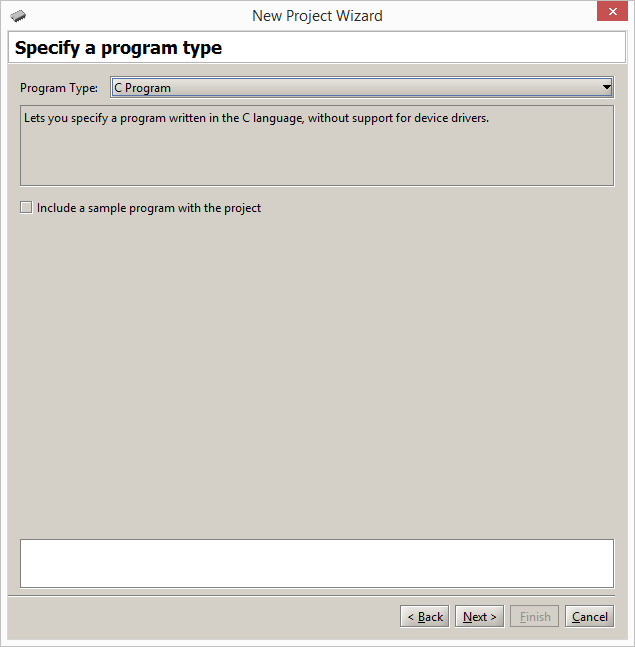
\includegraphics[scale=0.58]{figures/figureMP_progtype.png}
	\end{center}
	\vspace{-0.25cm}\caption{Setting the program type.}
\label{fig:MPprogtype}
\end{figure}
\begin{figure}[H]
	\begin{center}
	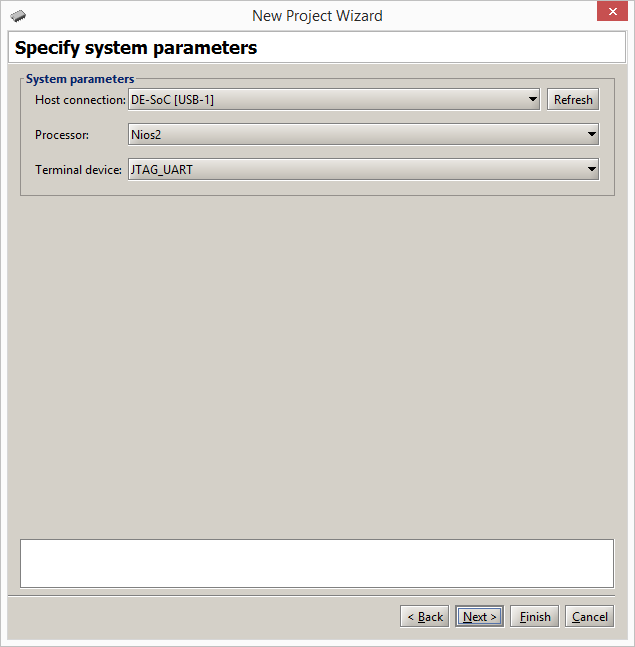
\includegraphics[scale=0.58]{figures/figureMP_terminal.png}
	\end{center}
	\vspace{-0.25cm}\caption{Configuring the {\it Terminal} window.}
\label{fig:MPterminal}
\end{figure}

\begin{figure}[H]
	\begin{center}
	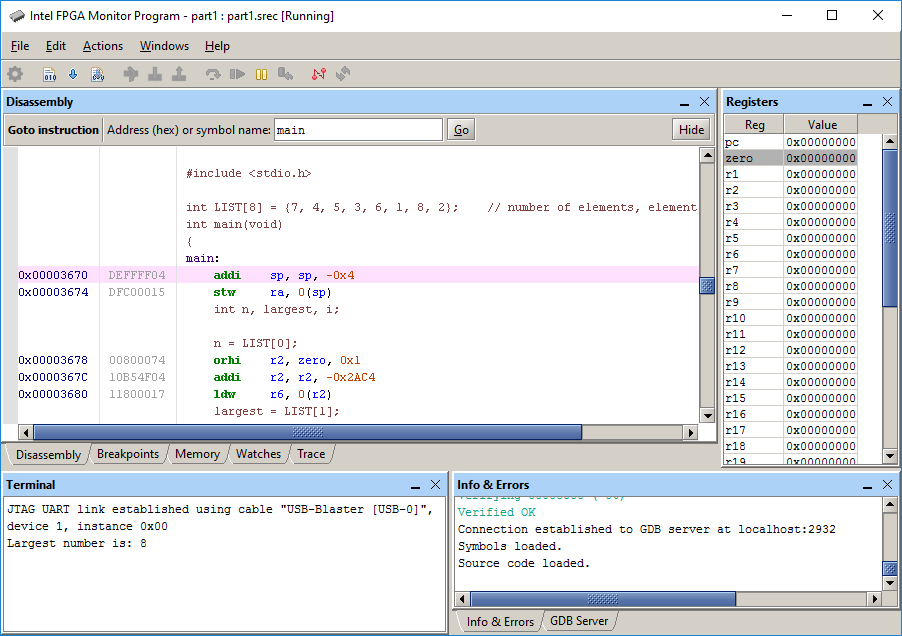
\includegraphics[scale=0.58]{figures/figureMP_goto.png}
	\end{center}
	\caption{Displaying the code for the C program.}
\label{fig:MPgoto}
\end{figure}

\section*{Part II}
\addcontentsline{toc}{2}{Part II}
Using the {\it printf} function results in a fairly large number of assembly-language instructions,
because the standard library routines are quite complex. Modify your program to display the 
result on the red lights {\it LEDR}, instead of using the {\it printf} statement. The
parallel port in the computer systems is connected to the red lights is memory-mapped at the 
address {\sf 0xFF200000}, as illustrated in Figure~\ref{fig:LEDR}.

~\\
Compile, download, and run this program. Observe the difference in the size of the
machine code for this program as compared to the one from Part I.

\begin{figure}[H]
	\begin{center}
	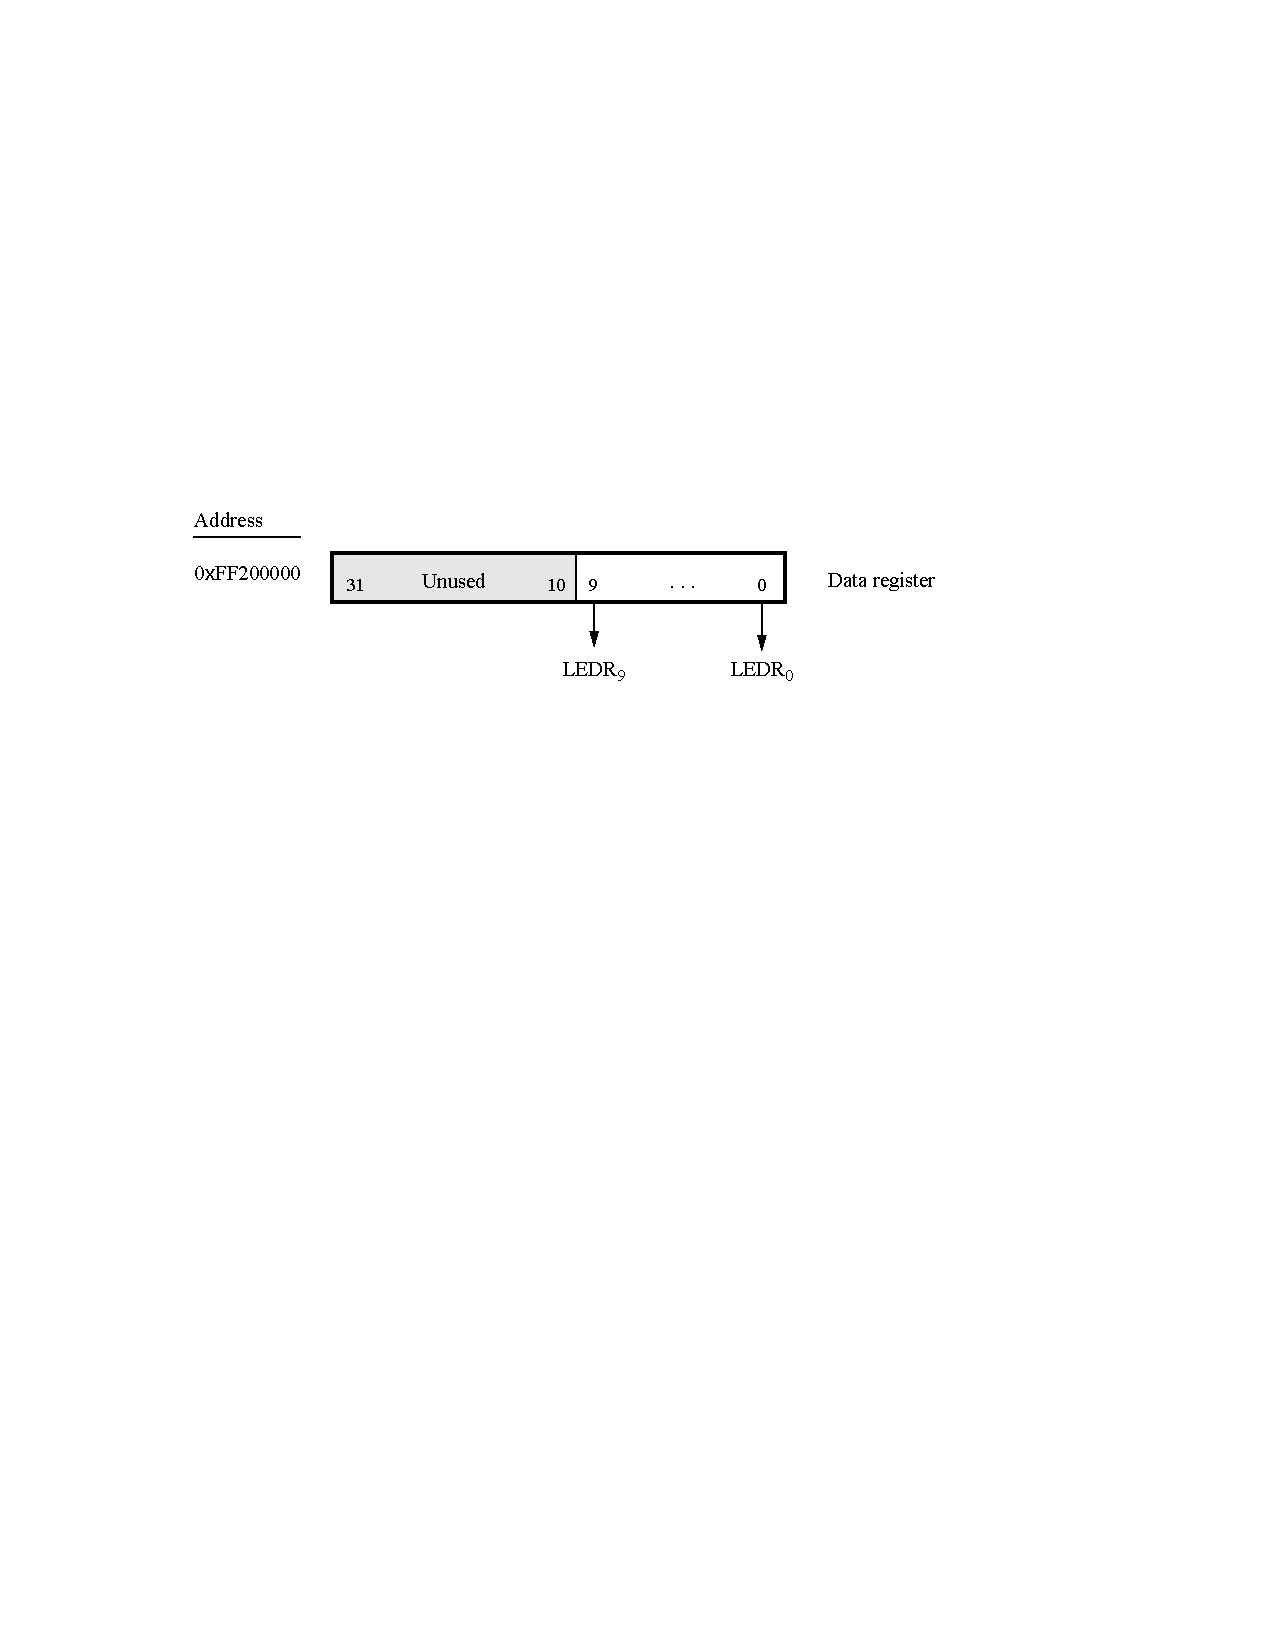
\includegraphics[scale=.7]{figures/figureLEDR.pdf}
	\end{center}
	\caption{The parallel port connection to the red lights.}
\label{fig:LEDR}
\end{figure}


\section*{Part III}
\addcontentsline{toc}{3}{Part III}
In Exercise 2, you were given a program that uses shift and AND operations to find the
longest string of 1's in a word of data. The program is reproduced in
Figure~\ref{fig:shiftAND}.  In Parts III and IV of Exercise 2, you were asked to extend
this program so that it processed a list of data words, rather than just one word. Also,
the program was extended to compute the longest
strings of 1's, the longest string of 0's, and the longest string of alternating 1's and 0's
for any of the words in the list. The results of these computations were to be shown 
on the 7-segment displays of the computer. For this part of the exercise, you are 
to write a C-language program to implement these tasks.

\begin{figure}[H]
\begin{center}
\lstinputlisting[style=defaultNiosStyle]{../design_files/part3.s}
\end{center}
\caption{Assembly-language program that counts consecutive ones.}
\label{fig:shiftAND}
\end{figure}

To include the list of data words in your C program, you can declare them as an array using
a statement such as

\begin{lstlisting}[language=C]
int TEST_NUM[ ] = {0x0000e000, 0x3fabedef, 0x00000001, 0x00000002, 0x75a5a5a5,
                   0x01ffC000, 0x03ffC000, 0x55555555, 0x77777777, 0x08888888,
                   0x00000000};
\end{lstlisting}


Display the count for the longest string of 1's on 7-segment displays {\it HEX}$1-0$, 
for the longest string of 0's on {\it HEX}$3-2$, and for 
alternating 1's and 0's on {\it HEX}$5-4$. 
The parallel ports connected to the 7-segment displays in the computer systems
are illustrated in Figure~\ref{fig:HEX}.

\begin{figure}[H]
	\begin{center}
	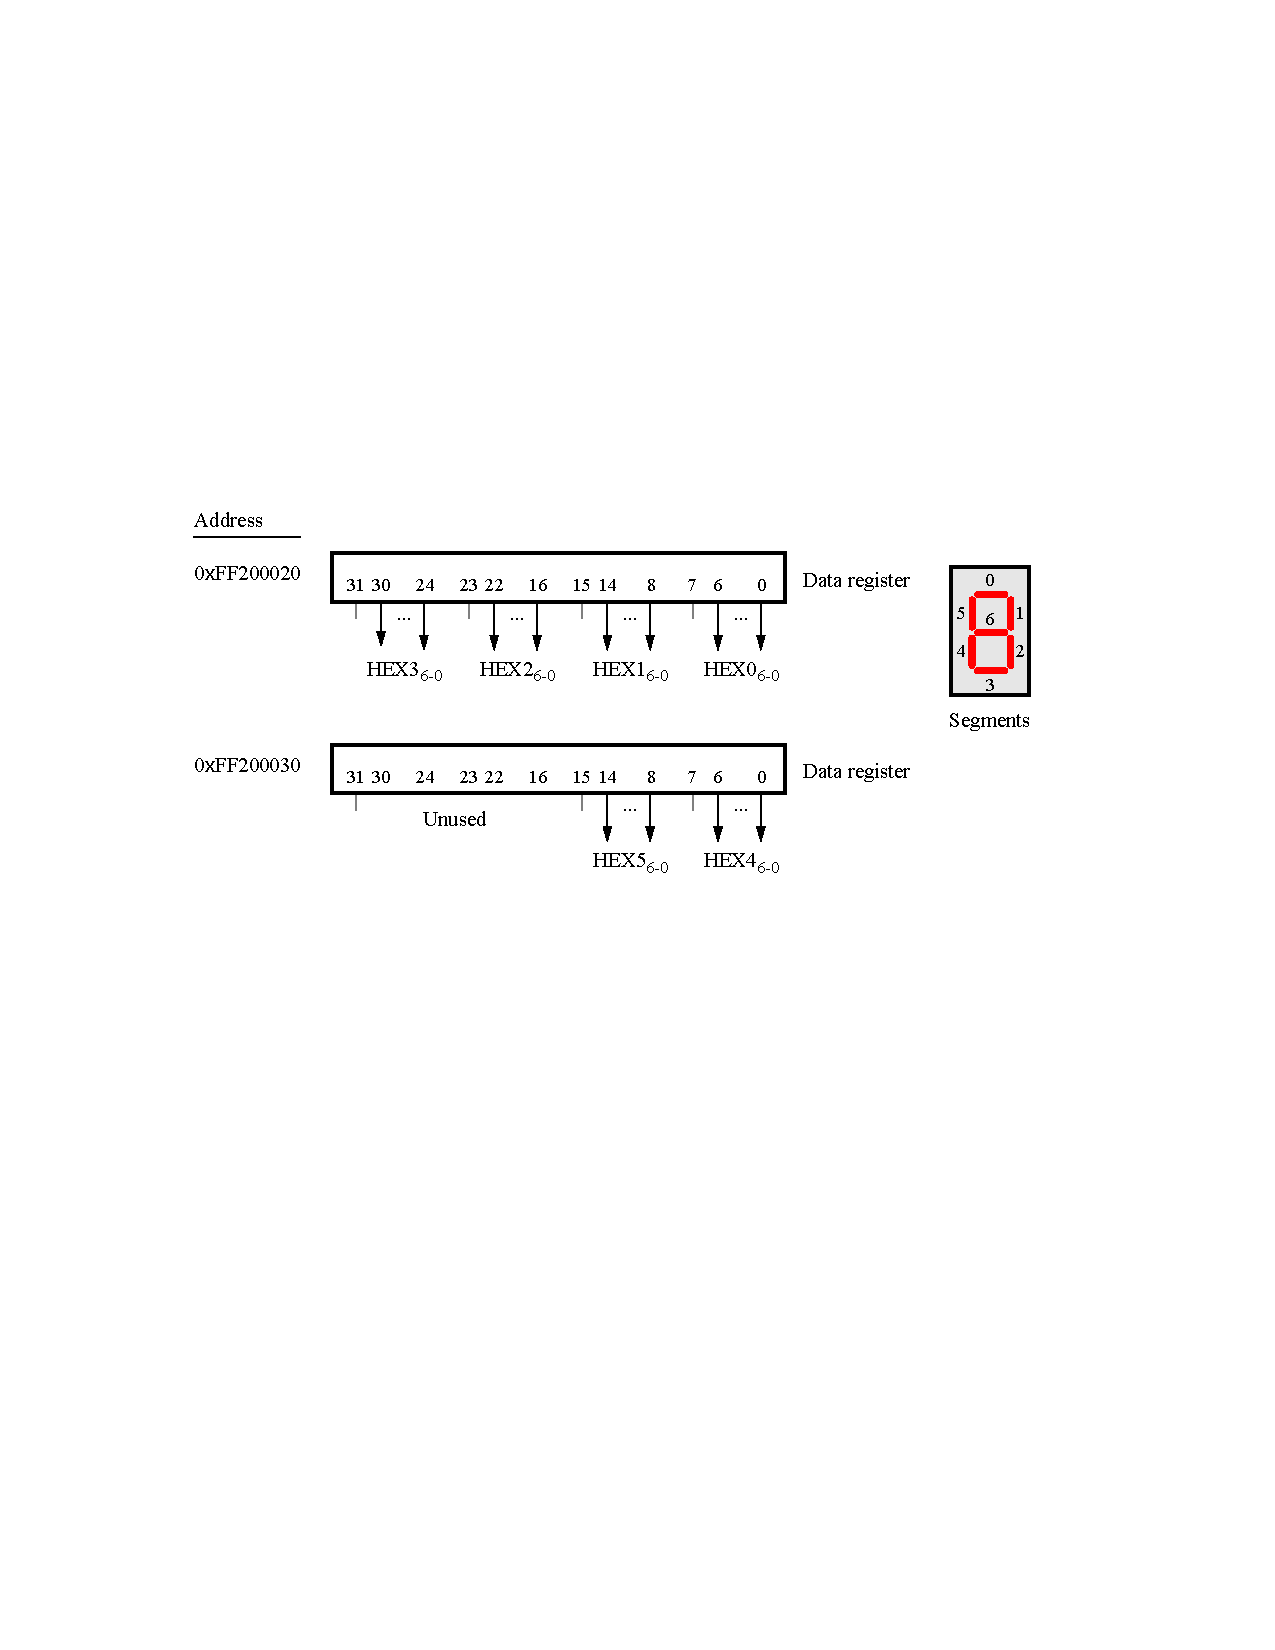
\includegraphics[scale=.8]{figures/figureHEX.pdf}
	\end{center}
	\caption{The parallel ports connected to the 7-segment displays.}
\label{fig:HEX}
\end{figure}

Create a new folder and Monitor Program project for your C program, and then compile,
download, and test the code. Using the ten words of test data shown above, the correct
result that should appear on the {\it HEX}$5-0$ displays is \red{\sf 32 31 12}.

\section*{Part IV}
\addcontentsline{toc}{4}{Part IV}
In Exercise 4 you were asked to implement a real-time clock in the Computer System. The
clock-time was shown on the {\it HEX}$3-0$ seven-segment displays in the format \red{SS}:\red{DD},
with \red{\it SS} representing seconds and \red{\it DD} representing hundredths of a second.
Time was measured in intervals of 0.01 seconds by using polled I/O with the Interval Timer, 
and the clock could be stopped/run by pressing one of the pushbutton {\it KEYs}.

~\\
In this part of the exercise you are to write a C program that implements a real-time
clock. Display the clock-time on the 7-segment displays {\it HEX}$5-0$
in the format \red{MM}:\red{SS}:\red{DD}, where 
where \red{\it MM} are minutes, \red{\it SS} are seconds, and \red{\it DD} are hundredths of 
a second.  Measure time intervals of 0.01 seconds in your program by using polled I/O with the 
Interval Timer.  You should be able to stop/run the clock by pressing any pushbutton {\it KEY}.
When the clock reaches \red{59}:\red{59}:\red{99}, it should wrap around to
\red{00}:\red{00}:\red{00}.

~\\
Make a new folder to hold your Monitor Program project for this part. Create a
file called {\it part4.c} and type your C code into this file.  Make a new Monitor Program 
project for this part of the exercise, and then compile, download, and test your program. 


\section*{Part V}
\addcontentsline{toc}{5}{Part V}
Write a C program that scrolls the word \red{\sf intEL}
in the right-to-left direction across the 7-segment displays.
An example of the scrolling behaviour is given in Table~\ref{tab:scrolling}.
You should scroll the display at a rate of 0.2 seconds per character. You should be able to stop/run the scrolling
message by pressing the {\it KEY} pushbuttons.

\begin{table}[H]
\begin{minipage}[t]{12.5 cm}
\begin{center}
\begin{tabular}{c|cccccc}
Time slot & \multicolumn{6}{c}{Display} \\
\hline
{\rule[0mm]{0mm}{5mm}0} &\red{i}&\red{n}&\red{t}&\red{E}&\red{L}& \\ 
1 &\red{n}&\red{t}&\red{E}&\red{L}& & \\
2 &\red{t}&\red{E}&\red{L}& & & \\
3 &\red{E}&\red{L}& & & & \\
4 &\red{L}& & & & & \\
5 & & & & & & \\
6 & & & & & &\red{i}\\
7 & & & & &\red{i}&\red{n}\\
$\ldots$ & & &$\ldots$ & &\\
\end{tabular}
\caption{Scrolling the message \red{\sf intEL} on {\it HEX}$5-0$.}
\label{tab:scrolling}
\end{center}
\end{minipage}
\end{table}

Note that scrolling a message across the 7-segment displays is similar in nature to the 
task of implementing a real-time clock, from Part IV. You should be able to reuse most of 
your code from Part IV. But instead of updating the clock each time the Interval Timer
expires, you need to update the scrolling message.  

~\\
Make a new folder to hold your Monitor Program project for this part. Create a
file called {\it part5.c} and type your C code into this file.  Make a new Monitor Program 
project, compile, download, and test your program. 




%%%%%%%%%%%%%%%%%%%%%%%%%%%%%%%%%%%%%%%%
%%% FPGAcademy Copyright Information %%%
%%%%%%%%%%%%%%%%%%%%%%%%%%%%%%%%%%%%%%%%

%Always put the copyright on a new page (clear page), with some vertical space from top
\clearpage
\vspace{1in}

\noindent

Copyright {\copyright} FPGAcademy.org. All rights reserved. FPGAcademy and the 
FPGAcademy logo are trademarks of FPGAcademy.org.  This document is provided 
"as is", without warranty of any kind, express or implied, including but not 
limited to the warranties of merchantability, fitness for a particular purpose 
and noninfringement. In no event shall the authors or copyright holders be 
liable for any claim, damages or other liability, whether in an action of 
contract, tort or otherwise, arising from, out of or in connection with the 
document or the use or other dealings in the document.
~\\
~\\
**Other names and brands may be claimed as the property of others.


\end{document}
